\documentclass[a4paper,12pt]{article}
\usepackage[utf8]{inputenc}
\usepackage[spanish]{babel}
\usepackage{microtype}

\usepackage{graphicx}
\usepackage{wrapfig}

\usepackage{amssymb}
\usepackage{amsmath} %For being able to make comments inside the formulas as normal text
\usepackage{amsthm}
\usepackage{float}
\usepackage{cancel} %in the preamble gives you four different modes of striking through

\usepackage[a4paper, inner= 2cm, outer= 2cm,
top= 2cm, bottom= 2cm]{geometry}
\usepackage{fancyhdr}
\usepackage{animate}
\usepackage{hyperref}
\usepackage{listings}

\providecommand{\abs}[1]{\lvert#1\rvert}
\providecommand{\norm}[1]{\lVert#1\rVert}



\lstdefinestyle{mystyle}{
    backgroundcolor=\color{backcolour},   
    commentstyle=\color{codegreen},
    keywordstyle=\color{magenta},
    numberstyle=\tiny\color{codegray},
    stringstyle=\color{codepurple},
    basicstyle=\ttfamily\footnotesize,
    breakatwhitespace=false,         
    breaklines=true,                 
    captionpos=b,                    
    keepspaces=true,                 
    numbers=left,                    
    numbersep=5pt,                  
    showspaces=false,                
    showstringspaces=false,
    showtabs=false,                  
    tabsize=2
}




\usepackage[dvipsnames]{xcolor}
\definecolor{blueMacc}{RGB}{61, 160, 250}

\title{{\color{blueMacc}Taller 3}}
\author{David Alsina, Juan Luis Ávila, Juan Andrés Guevara y Jairo Gudiño}
\date{Marzo 2021}


\begin{document}

    \begin{figure}[ht]
        \centering
        \includegraphics[width = \linewidth]{Header.png}
        \maketitle
    \end{figure}

    \section{Introducción}
        En el presente reporte buscamos dar solución a diversos problemas relacionados con la proyección de números complejos sobre la esfera de Riemman (proyección estereográfica). Específicamente, resolvemos el problema de proyectar gráficas no triviales y la construcción de $app$ para proyectar una serie de líneas, dado un conjunto de puntos definidos como entradas secuenciales por el usuario. 
    
    \section{Solución del problema}
    
    \begin{enumerate}
        \item \textit{Proyección de gráficas no triviales sobre la esfera de Riemman:} 
        
        Utilizando la función $sphere$, recreamos una esfera en 3D para representar allí los puntos en el plano de los complejos. A continuación, utilizamos la función $RectangularToSphere$ que convierte las coordenadas en el plano en puntos sobre la esfera para obtener las gráficas dentro de ésta última. Con las coordenadas obtenidas, utilizamos la función $plot3$ para representar los outputs de distintas funciones matemáticas ($createSpirographCoordinates$, $createArchimedeanSpiralCoords$, $createHipocicloidCoordinates$).
        
        Para obtener las gráficas en 2D, utilizamos estas mismas funciones matemáticas definidas anteriormente pero graficamos los resultados utilizando la función $graphComplexDomain$. 
        
        Las funciones matemáticas fueron construidas por cada uno de los integrantes así como su representación final en el plano de los complejos y en la esfera, pero las funciones para ésto último fueron desarrolladas por David Alsina.
        
        \item \textit{Proyección de lineas generadas a partir de entradas de usuario:}
        
        Como se describe en la siguiente sección de pseudo-código, a medida que el usuario va definiendo los puntos que le interesan, mediante el código de la interfaz se van graficando los puntos de acuerdo con el orden en el que aparecen. Los puntos son unidos mediante la función $f_unir_puntos_interfaz$, mientras que la graficación de las proyecciones estereográficas, que se hace al final, se realiza mediante la función $graphProyectionInRiemmanSphereGUI$.
        
        El desarrollo de ésta parte la hizo Juan Andrés junto con David Alsina.
        
    \end{enumerate}
    
    \section{El pseudocódigo}
    
    \begin{enumerate}
        \item \textit{Proyección de gráficas no triviales sobre la esfera de Riemman:} 
        
        \begin{enumerate}

            \item Creación de funciones para graficar el dominio (figura no trivial en el plano complejo, ej: un hipocloide). 
            \item Creación de funciones para proyección de una serie de puntos en el plano complejo sobre la esfera de Riemman.
            
            \item Construcción de funciones generadoras de la serie de puntos (a proyectar) que conforman las gráficas de los dominios.
            
            \item Graficación de la serie de puntos (creados con la función mencionada en el item \textit{(c)})  usando la función construida en el item \textit{(a)}, y graficación de su correspondiente proyección sobre la esfera, usando la función de  \textit{(b)}.
        \end{enumerate}
        
        \item \textit{Proyección de lineas generadas a partir de entradas de usuario:}
        
        \begin{enumerate}
            \item Primero definimos unos ejes en la aplicación que permitan al usuario seleccionar puntos en el mismo, usando el método \emph{ginput}.
            
            \item Una vez el usuario haya seleccionado los puntos de interés, estos se graficarán en los ejes anteriormente creados usando el método \emph{plot}, el cuál unirá los puntos en el orden en que estos se vayan graficando.
            
            \item Definimos nuevamente otros ejes, para graficar la proyección estereográfica de la entrada del usuario.
            
            \item Parametrizamos las líneas formadas por la unión de los puntos para obtener los puntos que están sobre las líneas.
            
            \item Realizamos la proyección estereográfica a todos los puntos obtenidos anteriormente y graficamos con el método \emph{plot3}.
            
        \end{enumerate}
    \end{enumerate}
  
    \newpage
    
    \section{Figuras y conclusiones}
    
    \subsection{Espirales de Arquímides}
    
    Las espirales de arquímedes \footnote{\textcolor{blueMacc}{\underline{\href{https://es.wikipedia.org/wiki/Espiral_de_Arqu\%C3\%ADmedes}{Espirales de Arquímedes.}}}} se construyen a partir de la fórmula: 
    
    \begin{equation*}
        r = a + b\theta
    \end{equation*}
    
    \begin{figure}[H]
        \centering
        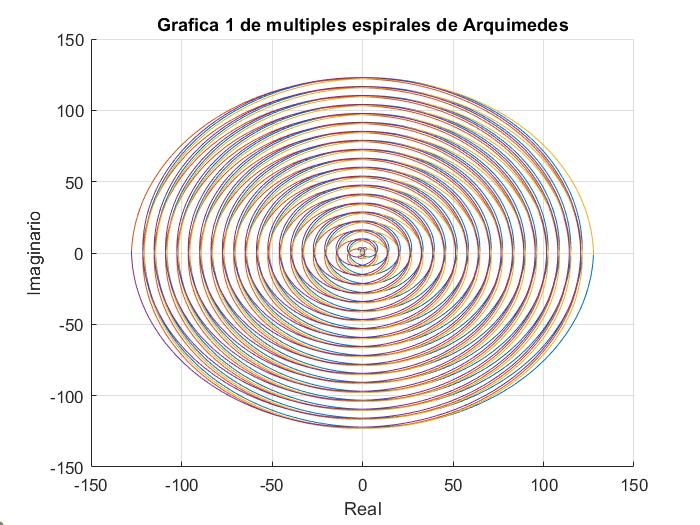
\includegraphics[width=0.49\linewidth]{grafica1EspiralesArquimedes_no_zoom.jpg}\\
        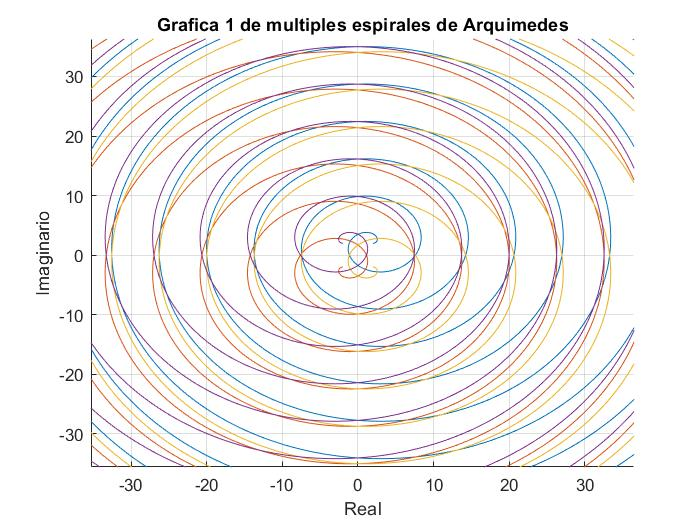
\includegraphics[width=0.49\linewidth]{grafica1EspiralesArquimedes_zoom_med.jpg}
        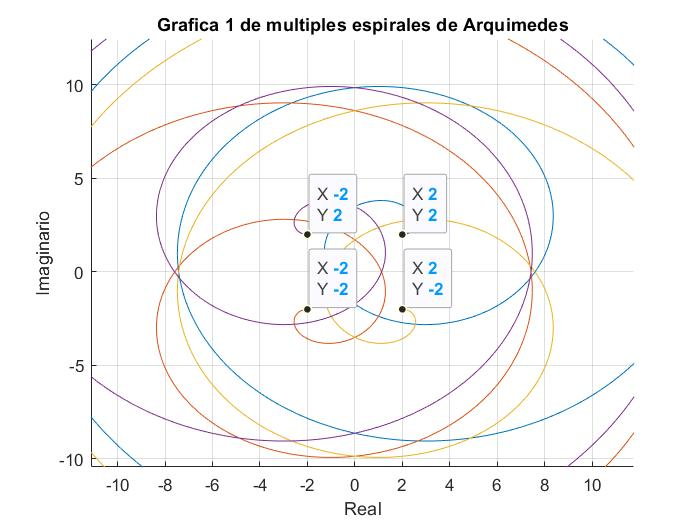
\includegraphics[width=0.49\linewidth]{grafica1EspiralesArquimedes_zoom.jpg}
        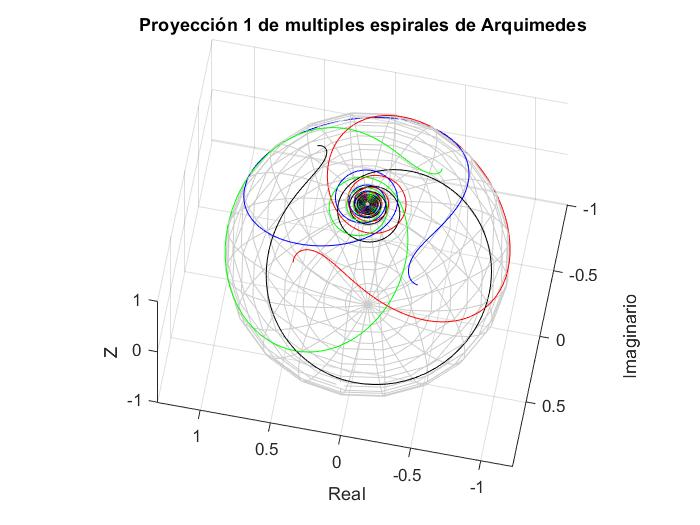
\includegraphics[width=0.49\linewidth]{grafica1EspiralesArquimedes_proyect1.jpg}
        \caption{Domino con centro distinto (3 imagenes con distintos niveles de zoom) y su respectiva proyección.}
    \end{figure}
    
    \begin{figure}[H]
        \centering
        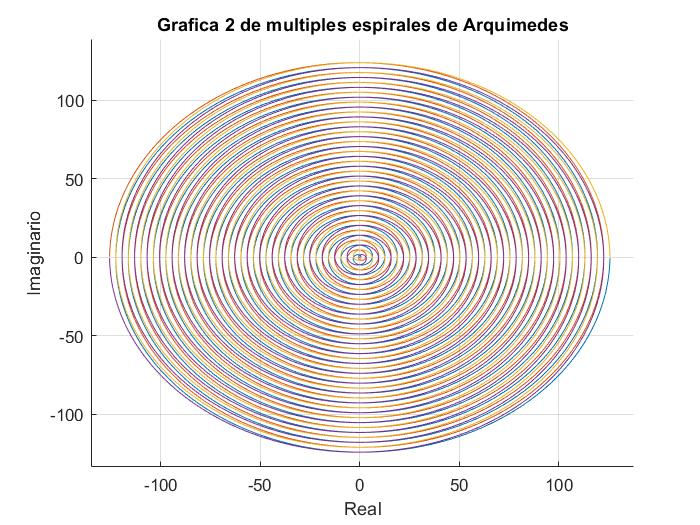
\includegraphics[width=0.49\linewidth]{grafica2EspiralesArquimedes_no_zoom.jpg}\\
        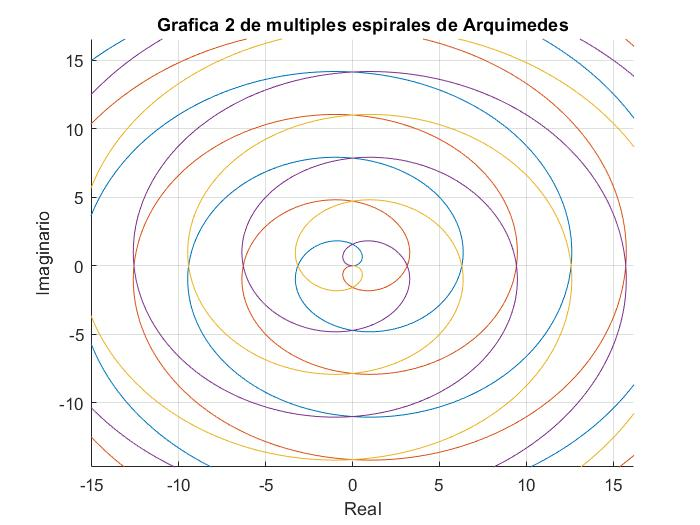
\includegraphics[width=0.49\linewidth]{grafica2EspiralesArquimedes_zoom_med.jpg}
        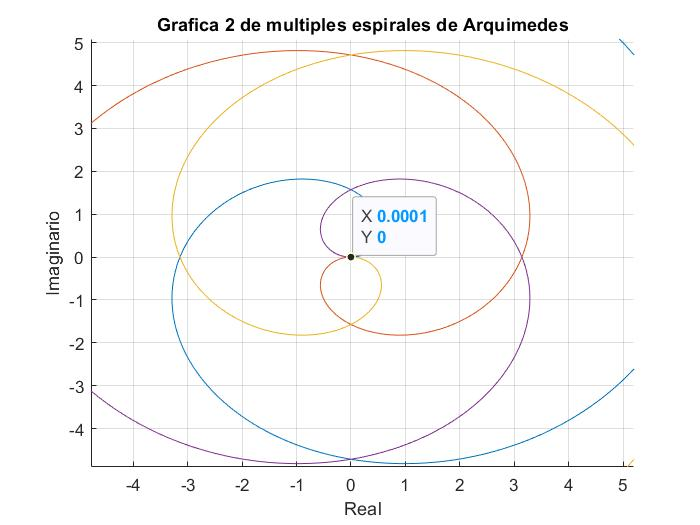
\includegraphics[width=0.49\linewidth]{grafica2EspiralesArquimedes_zoom.jpg}
        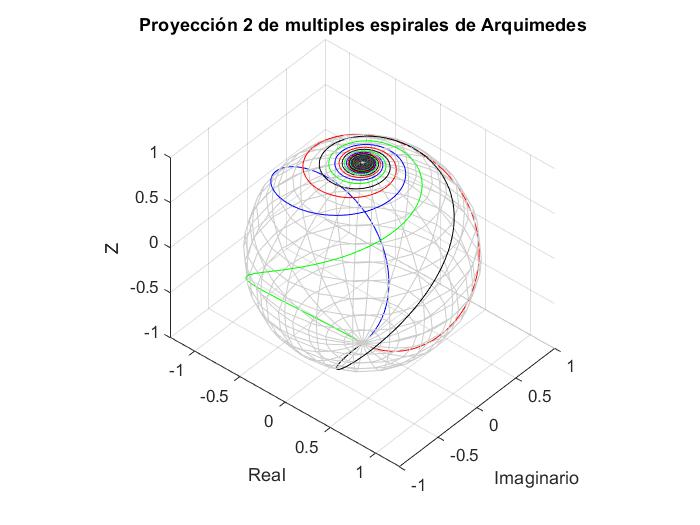
\includegraphics[width=0.49\linewidth]{grafica2EspiralesArquimedes_proyect1.jpg}
        \caption{Domino de espirales de arquimedes con mismo centro (3 imagenes con distintos niveles de zoom) y su respectiva proyección.}
    \end{figure}
    
    \newpage
    %--------------
    \subsection{Rosas polares}
    Se realizó la simulación y las respectivas gráficas con rosas polares de la forma:
    
    \begin{equation*}
        r(\theta) = a(\sin(5\theta))
    \end{equation*}
    
    con distintos valores de $a$.\footnote{\textcolor{blueMacc}{\underline{\href{https://es.wikipedia.org/wiki/Rosa_polar}{Rosas Polares.}}}}
    
    \begin{figure}[H]
        \centering
        \includegraphics[width=0.47\linewidth]{jl_plano_complejo,png.png}
        \includegraphics[width=0.52\linewidth]{jl_unitario.png}
        \includegraphics[width=0.6\linewidth]{jl_riemann.png}
        \caption{Vista de múltiples rosas polares en el plano complejo y en la esfera de Riemann.}
        \label{polares}
    \end{figure}
    
    
    
    \newpage
    %--------------
    \subsection{Espirógrafos}
    Se realizó la simulación y las respectivas gráficas de múltiples espirógrafos en un mismo gráfico del plano de los complejos, construyendo cada uno con distintos valores de $b$ desde 8 hasta 15 que satisfacen las siguientes ecuaciones para $x$ y $y$:
    
    \begin{align*}
        x(\theta) = (a-b)\cos \theta + d \cos \frac{a-b}{b} \theta \\
        y(\theta) = (a-b)\sin \theta - d \sin \frac{a-b}{b} \theta
    \end{align*}
    
    En la simulación, los valores de $theta$ dependen de $b$, al variar dentro de un rango desde 0.01 hasta $ \frac{2b \pi}{m.c.m(a,b)}$ avanzando en 0.01 unidades, donde $m.c.m$ denota mínimo común múltiplo. Los valores de $a$ y $d$ fueron fijados en 16 y 7 respectivamente.
    
    \begin{figure}[H]
        \centering
        \includegraphics[width=0.47\linewidth, height=7cm]{esp_1.PNG}
        \includegraphics[width=0.52\linewidth, height=7cm]{esp_2.PNG}
        \includegraphics[width=0.6\linewidth, height=7cm]{esp_3.PNG}
        \caption{Vista de múltiples espirógrafos en el plano complejo y en la esfera de Riemann.}
        \label{polares}
    \end{figure}
    
    \footnote{\textcolor{blueMacc}{\underline{\href{https://en.wikipedia.org/wiki/Spirograph}{Espirógrafos.}}}} 
    
    \newpage
    \subsection{Hipocicloides}
    Se graficaron hipocilcloides\footnote{\textcolor{blueMacc}{\underline{\href{https://en.wikipedia.org/wiki/Hypocycloid}{Hipocicloides.}}}}, las cuales son curvas que satisfacen las siguientes ecuaciones paramétricas:
    
    \begin{align*}
        x(\theta) = r(k-1)\cos \theta + r \cos ((k-1)\theta) \\
        y(\theta) = r(k-1)\sin \theta - r \sin ((k-1)\theta)
    \end{align*}
    
    En particular se tomaron los parámetros $k = 2.1$, $r = 1$ y $0 < \theta < 20\pi$.
    
    \begin{figure}[H]
        \centering
        \includegraphics[width=0.49 \linewidth]{hipoDomain.png}
        %\caption{Caption}
        %\label{fig:my_label}
        \includegraphics[width=0.49\linewidth]{hipoInSphereView2.png}
        \includegraphics[width=0.65\linewidth]{hipoInSphere.png}
    \end{figure}
    
    \subsection{Conclusiones}
    Proyectando distintas figuras que se pueden hacer en el plano de los números complejos sobre la esfera de Riemann se obtienen no sólo gráficos artísticamente interesantes como mandalas con los espirógrafos, sino también representaciones dinámicas de trayectorias como se encontró con las espirales de Arquímedes, los hipocicloides y las rosas polares.
    
\end{document}
